\documentclass[12pt,a4paper]{ctexart}
\usepackage{amsmath,amssymb,bm}
\usepackage{graphicx}
\usepackage[margin=2.5cm]{geometry}
\usepackage{booktabs}
\usepackage{caption}
\usepackage{array}
\graphicspath{{figures/}}

\title{\textbf{计算机控制系统设计与实践\\ 第八周作业}}
\author{}
\date{}

\begin{document}
\maketitle

\noindent
姓\quad 名：\underline{\ 刘峻豪\ }\hspace{4em} 学\quad 号：\underline{\ 3230105220\ }\\[1.2ex]
专\quad 业：\underline{\ 自动化\ }\hspace{4em} 指导教师：\underline{\ 喻洁\ }

\bigskip
\hrule
\bigskip

\section{题目}
某景点需要设计一套基于 PLC 的（音乐）喷泉控制系统。喷泉包括 A、B 大小两组喷头，每组由
$6$ 个电磁阀分别控制 $6$ 个喷头（A1$\sim$A6，B1$\sim$B6）；A 组喷头由水泵 P1 供水，B 组喷头由
水泵 P2 供水。控制室设启动按钮 SB1 和停止按钮 SB2（均为无自锁的点动按钮）。

\medskip
\noindent\textbf{控制要求：}
\begin{enumerate}
  \item 按下启动按钮 SB1 后，系统按下述时序循环运行：
  \begin{enumerate}
    \item 水泵 P1 打开，A 组 $6$ 个电磁阀门全开，喷 $6\,\mathrm{s}$ 后停止；
    \item 水泵 P2 打开，B 组 $6$ 个电磁阀门全开，喷 $6\,\mathrm{s}$ 后停止；
    \item A、B 两组喷头同时打开，喷 $6\,\mathrm{s}$ 后同时停止；
    \item 等待 $3\,\mathrm{s}$ 后，循环重复前述过程。
  \end{enumerate}
  \item 按下停止按钮 SB2 后，两组喷头同时停止喷水。
\end{enumerate}

\section{I/O 地址分配}
按题目给定的地址表，输入、输出点分配如表~\ref{tab:io} 所示。系统共 $2$ 个数字量输入、
$16$ 个数字量输出（$2$ 台水泵 $+\,7+7$ 路电磁阀，本题 A、B 组各按 $7$ 个连续位分配）。

\begin{table}[htbp]
  \centering
  \caption{喷泉控制系统 I/O 地址分配表}
  \label{tab:io}
  \renewcommand{\arraystretch}{1.25}
  \begin{tabular}{>{\centering\arraybackslash}p{3.2cm} >{\raggedright\arraybackslash}p{6.5cm} c}
    \toprule
    \textbf{地址} & \textbf{用途} & \textbf{类型} \\
    \midrule
    I0.0        & SB1 启动按钮        & 输入 \\
    I0.1        & SB2 停止按钮        & 输入 \\
    Q4.0        & 水泵 P1            & 输出 \\
    Q4.1        & 水泵 P2            & 输出 \\
    Q5.0$\sim$Q5.6 & A 组喷头电磁阀（A1$\sim$A6） & 输出 \\
    Q6.0$\sim$Q6.6 & B 组喷头电磁阀（B1$\sim$B6） & 输出 \\
    \bottomrule
  \end{tabular}
\end{table}

\section{控制策略与状态划分}
本题是典型的\textbf{顺序控制}问题：启动后按固定时序在若干工作状态之间自动切换，到时转移、
循环往复，直至停止。因此采用\textbf{顺序功能图（SFC）+ 起保停/置位复位}的设计方法：先用一个
\textbf{运行标志} M0.0 记录系统的启停（SB1 置位、SB2 复位，并自保持）；再把一个循环划分为
$4$ 个工作步，用辅助继电器 M2.0$\sim$M2.3 表示，各步的持续时间由定时器 T1$\sim$T4 控制。

\begin{table}[htbp]
  \centering
  \caption{工作步、标志、时间与输出对应关系（Q5为A组Q5.0$\sim$Q5.6，Q6为B组Q6.0$\sim$Q6.6）}
  \label{tab:steps}
  \renewcommand{\arraystretch}{1.3}
  \begin{tabular}{c c c c c c c}
    \toprule
    \textbf{工作步} & \textbf{标志} & \textbf{时间} & \textbf{P1(Q4.0)} & \textbf{P2(Q4.1)} & \textbf{A组(Q5)} & \textbf{B组(Q6)} \\
    \midrule
    步1 & M2.0 & 6\,s & ON  & OFF & ON  & OFF \\
    步2 & M2.1 & 6\,s & OFF & ON  & OFF & ON  \\
    步3 & M2.2 & 6\,s & ON  & ON  & ON  & ON  \\
    步4 & M2.3 & 3\,s & OFF & OFF & OFF & OFF \\
    \bottomrule
  \end{tabular}
\end{table}

\noindent 由表~\ref{tab:steps} 可得各输出的逻辑表达式：
\begin{equation}
Q4.0\,(\text{P1}) = Q5.0\!\sim\!Q5.6\,(\text{A 组}) = M2.0 + M2.2,
\end{equation}
\begin{equation}
Q4.1\,(\text{P2}) = Q6.0\!\sim\!Q6.6\,(\text{B 组}) = M2.1 + M2.2.
\end{equation}
即 A 组喷头与 P1 同步、B 组喷头与 P2 同步；步 3 两组同时喷水，步 4 全部停止形成 $3\,\mathrm{s}$ 间歇。

\section{顺序功能图（SFC）}
系统的顺序功能图如图~\ref{fig:sfc} 所示。上电处于初始步 S0（停机，全部输出为 $0$）；按下 SB1
后进入步 1，其后由定时器到时依次转移到步 2、步 3、步 4，步 4 延时 $3\,\mathrm{s}$ 到后返回步 1
形成循环。任何时刻按下 SB2 即复位运行标志与全部工作步，返回初始步 S0，两组喷头同时停喷。

\begin{figure}[htbp]
  \centering
  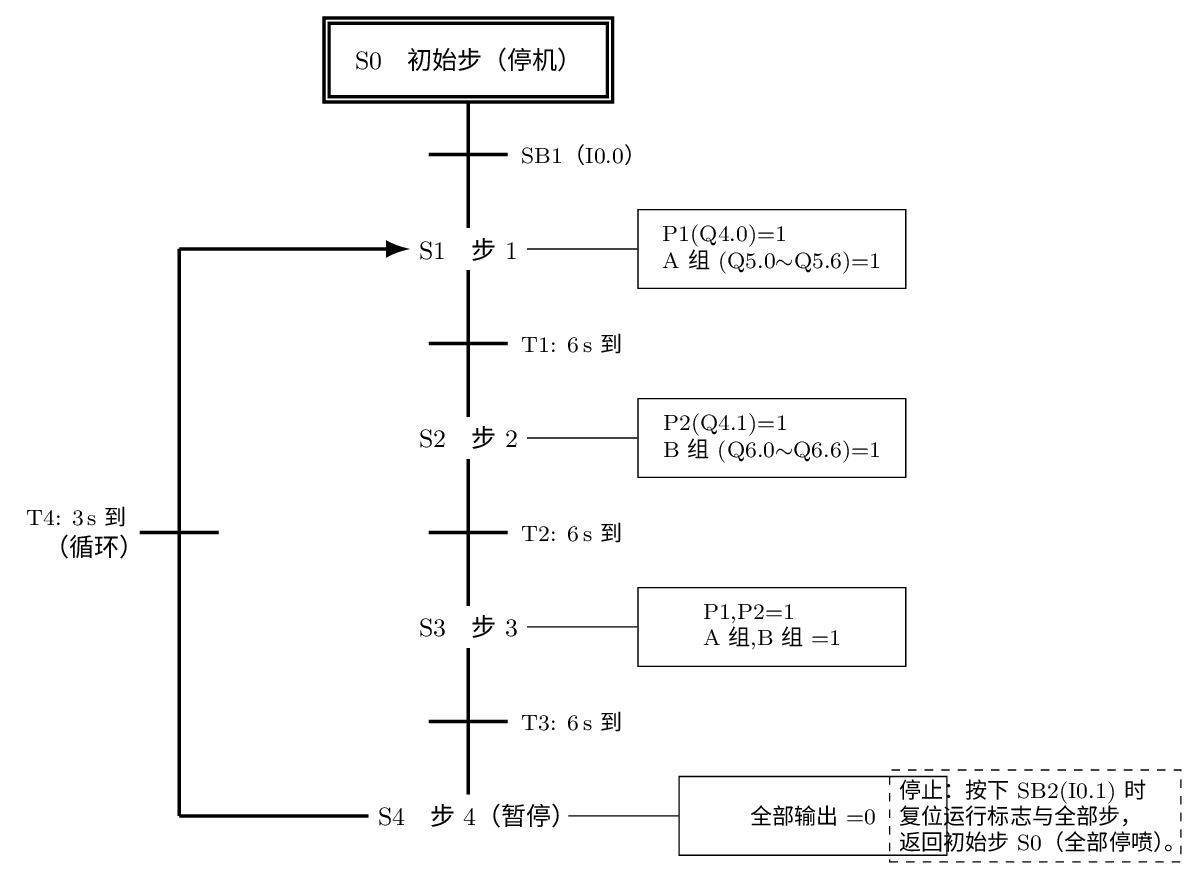
\includegraphics[width=0.86\linewidth]{sfc.png}
  \caption{音乐喷泉顺序控制系统的顺序功能图（SFC）}
  \label{fig:sfc}
\end{figure}

\section{梯形图程序设计}
根据 SFC，采用\textbf{置位（S）/复位（R）}指令实现工作步之间的转移，并用起保停电路实现运行
标志的自保持，梯形图分为两部分。

\subsection{运行标志与工作步转移}
如图~\ref{fig:ladderA}，网络 1 为运行标志 M0.0 的起保停电路：SB1（I0.0）接通使 M0.0 置位并
经其常开触点自保持，SB2（I0.1，常闭）断开则使 M0.0 及全部步复位。网络 2 定义初始工作步
M2.0：仅当系统运行（M0.0）且步 2$\sim$步 4 均未激活时成立。网络 3$\sim$8 用“上一步 + 本步定时器
到时”置位下一步、并复位上一步，实现单流程的顺序转移；网络 8 中 T4 到时复位步 4，使程序自动
回到步 1，实现循环。

\begin{figure}[htbp]
  \centering
  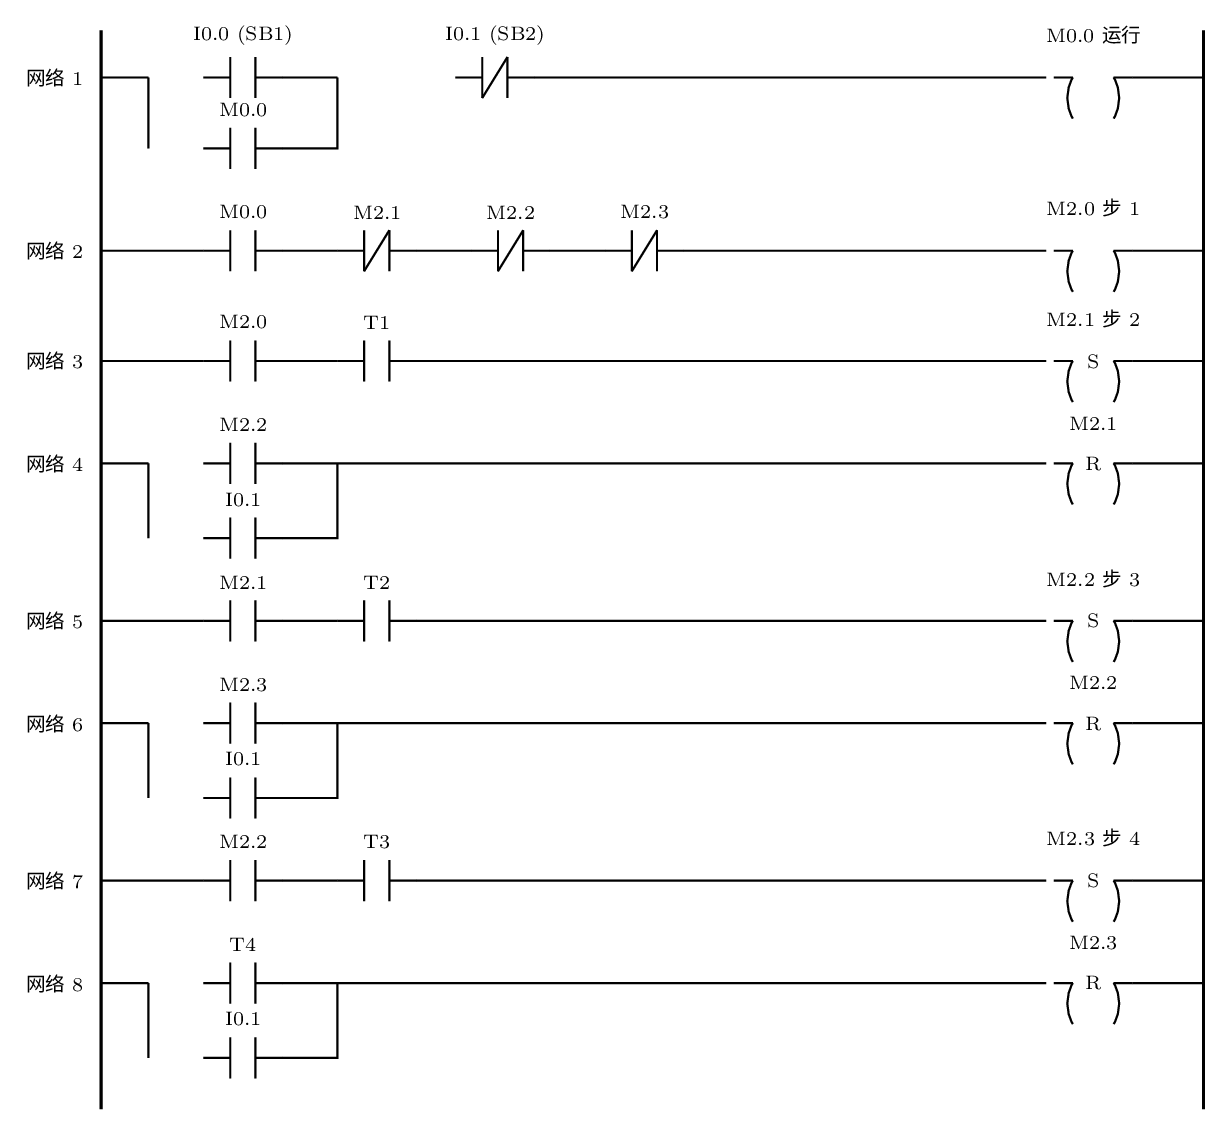
\includegraphics[width=0.98\linewidth]{ladderA.png}
  \caption{梯形图（一）：运行标志起保停与工作步 M2.0$\sim$M2.3 的顺序转移}
  \label{fig:ladderA}
\end{figure}

\subsection{定时器与输出驱动}
如图~\ref{fig:ladderB}，网络 9$\sim$12 分别由各工作步激活对应的接通延时定时器 T1$\sim$T4（前三步
$6\,\mathrm{s}$，第四步 $3\,\mathrm{s}$，西门子 S7 中以 \texttt{S5T\#6s}、\texttt{S5T\#3s} 设定）。
网络 13$\sim$16 按前述逻辑表达式驱动两台水泵和两组电磁阀：P1、A 组由“步 1 + 步 3”驱动，
P2、B 组由“步 2 + 步 3”驱动。

\begin{figure}[htbp]
  \centering
  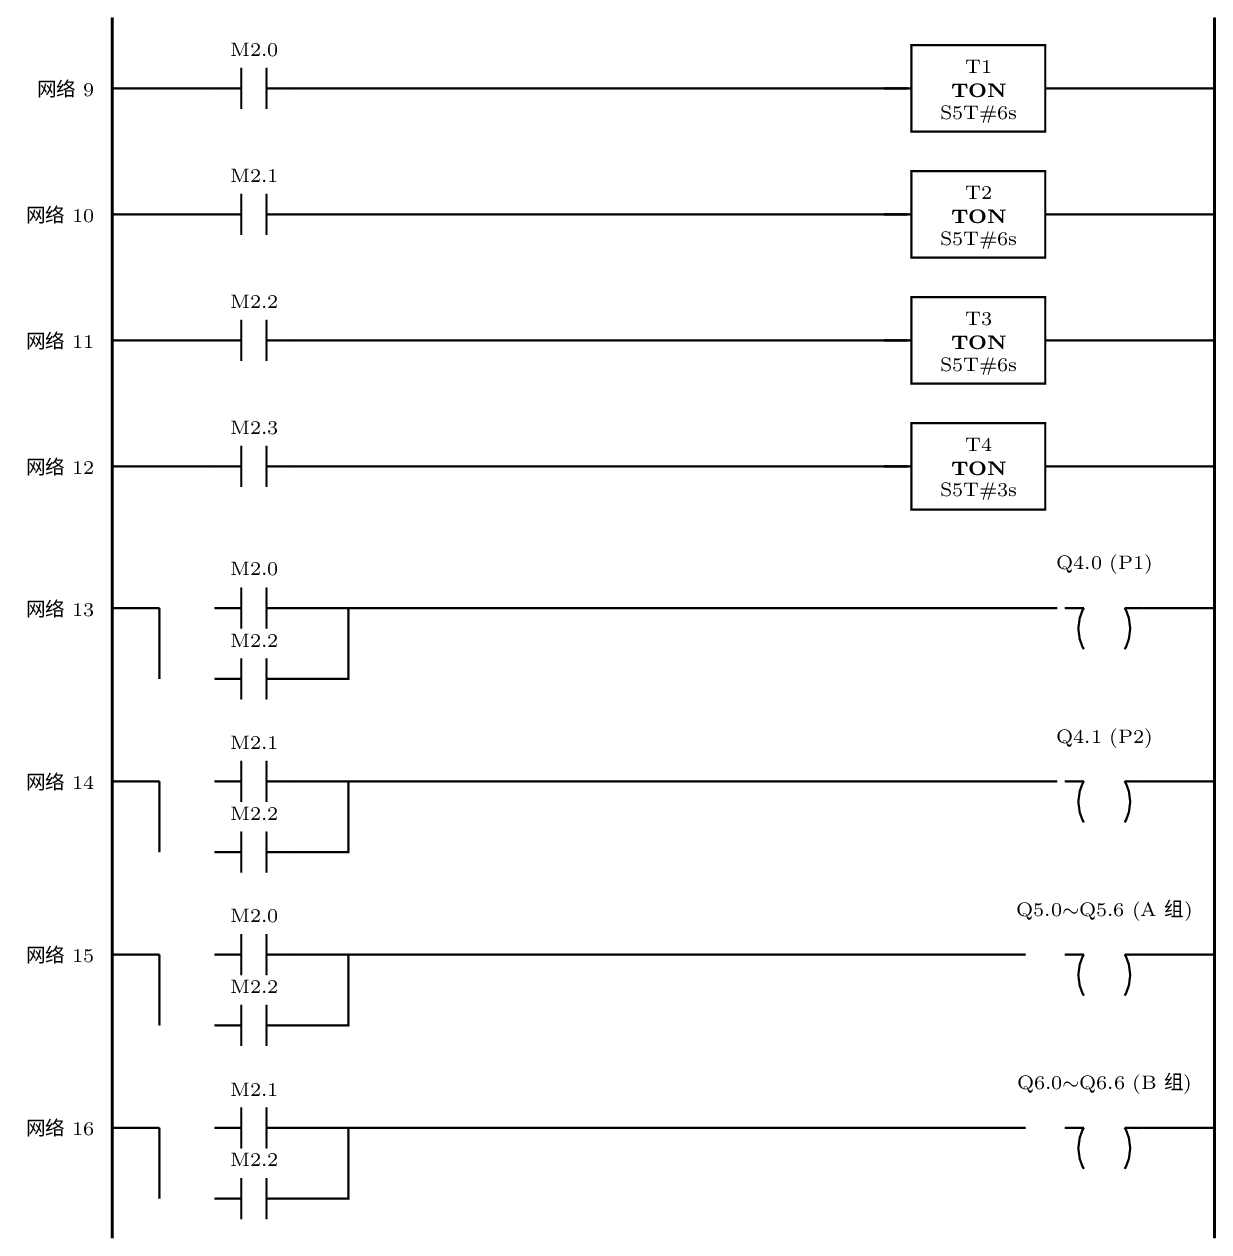
\includegraphics[width=0.98\linewidth]{ladderB.png}
  \caption{梯形图（二）：定时器 T1$\sim$T4 与水泵、电磁阀输出驱动}
  \label{fig:ladderB}
\end{figure}

\section{工作时序分析}
一个完整循环周期为 $T=6+6+6+3=21\,\mathrm{s}$。各输出的时序波形如图~\ref{fig:timing}：
步 1（$0\!\sim\!6\,\mathrm{s}$）P1 与 A 组为高；步 2（$6\!\sim\!12\,\mathrm{s}$）P2 与 B 组为高；
步 3（$12\!\sim\!18\,\mathrm{s}$）四路输出同时为高；步 4（$18\!\sim\!21\,\mathrm{s}$）全部为低，构成
$3\,\mathrm{s}$ 间歇，随后回到步 1 重复。停止时（SB2）无论处于哪一步都会立即将全部输出置 $0$。

\begin{figure}[htbp]
  \centering
  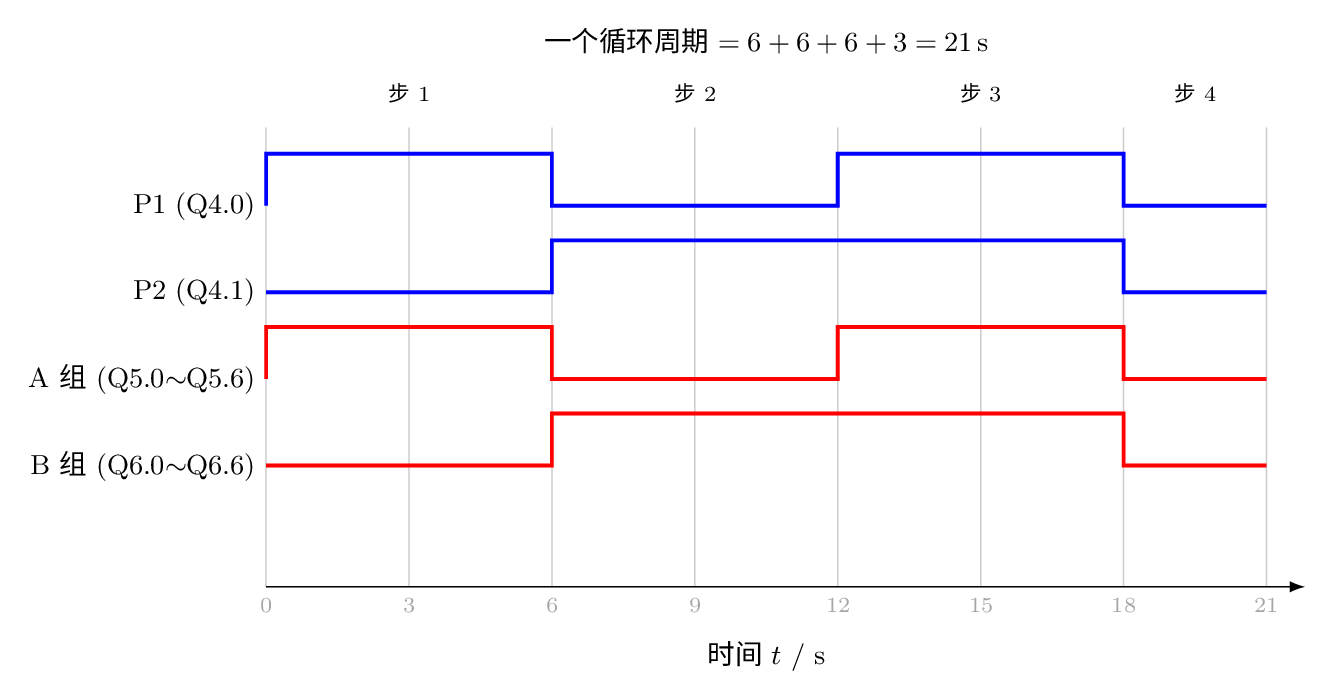
\includegraphics[width=0.95\linewidth]{timing.png}
  \caption{一个循环周期内各输出的工作时序图（周期 $21\,\mathrm{s}$）}
  \label{fig:timing}
\end{figure}

\section{扩展思考：按音乐节奏调节水泵开度}
若要求喷泉随音乐节奏改变喷水高度（水柱大小），则需把水泵由\textbf{开关（数字量）控制}升级为
\textbf{连续（模拟量）调速控制}，主要从以下几方面考虑：
\begin{enumerate}
  \item \textbf{执行机构}：将定速泵改为\textbf{变频器 + 交流电机}驱动，或采用比例调节阀/变量泵，
        通过改变转速或阀门开度连续调节流量与喷水高度。
  \item \textbf{控制量输出}：PLC 增加\textbf{模拟量输出模块（D/A）}，输出 $0\!\sim\!10\,\mathrm{V}$ 或
        $4\!\sim\!20\,\mathrm{mA}$ 信号作为变频器的频率给定，从而无级调节泵的“开度”。
  \item \textbf{音乐特征提取}：对音频信号进行采集与处理，提取\textbf{节拍（BPM）、节奏重音、
        频段能量（低/中/高音）与音量包络}等特征，作为控制的输入。可由上位机（PC/音频 DSP）完成
        FFT/包络分析，再经通信（如 Modbus/以太网 OPC）把特征值实时下传给 PLC。
  \item \textbf{映射与联动}：建立“音乐特征 $\rightarrow$ 频率给定”的映射曲线（如音量映射喷高、
        低频重拍触发大水柱、不同频段驱动不同喷头组），必要时加入\textbf{平滑滤波与限速}，
        避免开度突变造成水锤和电机冲击。
  \item \textbf{同步与实时性}：音乐、灯光与喷泉需时间同步，控制周期要足够小（如 $\le 50\,\mathrm{ms}$）
        以跟上节奏；可用预先编排的时间轴脚本保证重复演出的一致性。
  \item \textbf{安全与保护}：设置频率上下限、软启动/软停止、缺水与过载保护，防止低频长时间运行
        导致电机过热或水泵空转。
\end{enumerate}
综上，由开关量顺序控制升级为模拟量闭环/前馈控制，配合音频特征提取与合理的映射策略，即可实现
喷泉随音乐节奏动态调节水泵开度与喷水造型的效果。

\end{document}
